\section{Data processing and event selection}
\label{sec:data_processing}

\subsection{Sample waveforms and integration}

The RITA detection scheme yields distinct waveform topologies (Figure \ref{fig:waveforms}a,b)
depending on the emission direction of the \isotope{Th}{228} daughter isotopes. When an alpha
particle is emitted forward into the xenon gas, the recoiling daughter ion implants backward into
the silicon PIN diode (Figure \ref{fig:waveforms}d). By triggering the PMT channel at a high
threshold ($\sim$5 V)---effectively operating the chamber like a standard drift chamber with a
passive source---the corresponding $\sim$100 keV recoil implantation in the silicon can be clearly
observed in the coincident PIN signal.

However, the primary operation mode for active ion tagging relies on the reverse kinematics. The
system triggers on the large 4--8 MeV energy depositions of alpha particles striking the PIN
detector backward (Figure \ref{fig:waveforms}e). In this forward-recoil scenario, the daughter ion
travels into the active gas volume, generating a prompt S1 and a delayed S2 signal in the PMT
channel (Figure \ref{fig:waveforms}a,b). These S2 pulses possess much smaller amplitudes (typically
10--200 mV, dependent on $\Delta V_{\text{THGEM}}$) and a fixed drift time, as all ions originate
from the cathode surface.

\begin{figure}[t]
      \centering
      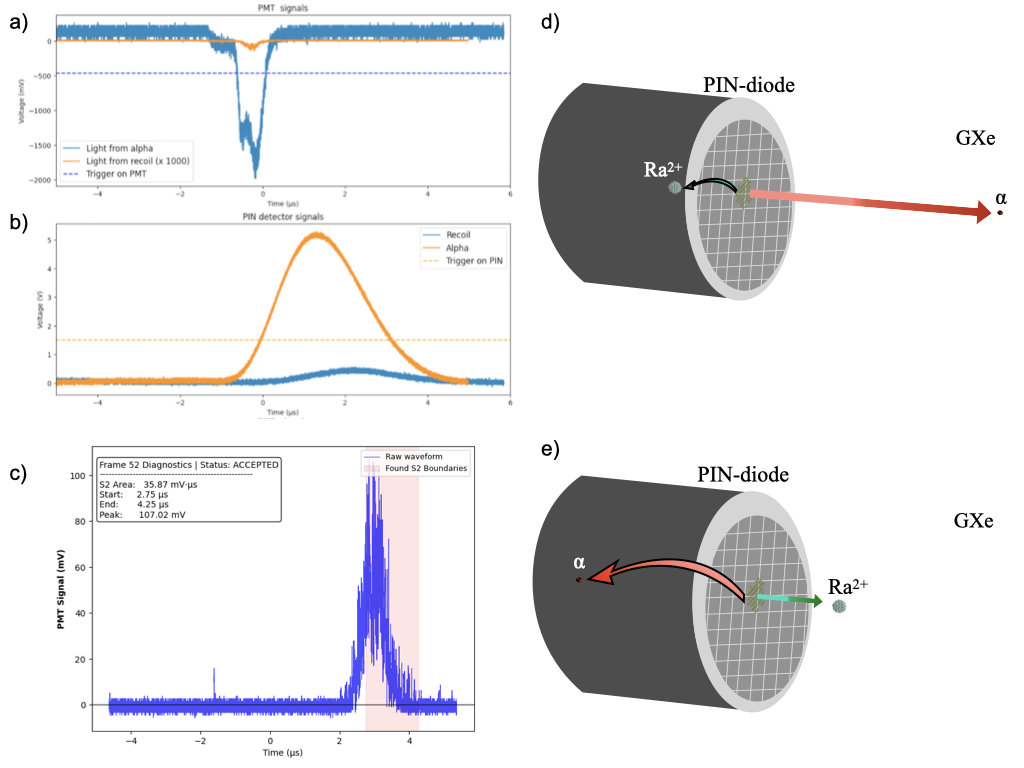
\includegraphics[width=0.95\textwidth]{figures/operation_modes.png}
      \caption{Waveform topologies and S2 integration methodology. (a, b) Characteristic signals in the PMT and PIN detectors under different trigger conditions. (c) A magnified view of the PMT channel demonstrating the delayed S2 pulse produced by a recoiling ion, highlighting the dynamically identified integration boundaries (shaded red). (d) Schematic representation of an alpha particle emitted forward into the xenon gas, resulting in a $\sim$100 keV backward recoil implantation into the PIN diode. (e) The primary active tagging mode: an alpha particle strikes the PIN detector backward, ejecting the recoiling daughter ion forward into the active gas volume to produce an S2 signal.}
      \label{fig:waveforms}
\end{figure}

To evaluate the ionization yield of the recoiling ions, the raw waveforms are processed offline.
The event selection process is strictly limited to checking for clipped events (which correspond to
alpha particles fully traversing the gas rather than recoils), applying a minimum voltage cut, and
restricting the signal integration to the S2 window, which is detected dynamically (Figure
\ref{fig:waveforms}c).

While the experimental hardware supports real-time gating via a single-channel analyzer (SCA), the
data presented in this analysis were acquired by triggering continuously across the full range of
alpha energies. This approach permits a simultaneous, multi-isotope analysis from a single dataset.
Individual events are classified offline by setting specific limits on the alpha energy peaks
recorded by the PIN detector.

\begin{figure}[t]
      \centering
      
\includegraphics[width=0.95\textwidth]{full_energy_spectrum.png}
      \caption{Full energy spectrum recorded by the silicon PIN detector. The data combine two trigger configurations to capture both the $\sim$100 keV recoil implantations (orange) and the high-energy 4--8 MeV alpha emissions (blue). The inset demonstrates the global energy linearity of the detector from the recoil scale up to the Po-212 alpha decay.}
      \label{fig:full_spectrum}
\end{figure}

\subsection{Event selection and isotopic tagging}

To comprehensively characterize the active source and validate the detector response, data were
acquired across the full energy range of the PIN diode. As shown in Figure \ref{fig:full_spectrum},
this spectrum encompasses both the low-energy $\sim$100 keV nuclear recoils (orange) and the
high-energy 4--8 MeV alpha emissions (blue). While capturing these two distinct populations
requires alternating the instrumental trigger configurations to accommodate the drastically
different signal amplitudes, the underlying emission kinematics within the active volume remain
physically identical. The inset in Figure \ref{fig:full_spectrum} demonstrates the robust global
linearity of the silicon detector across this broad dynamic range, confirming its fundamental
suitability for tracking the complete decay chain.

For the downstream analysis of recoil recombination physics, specific daughter isotopes must be
cleanly isolated. Because the hardware operates without a physical single-channel analyzer (SCA)
gate, this isotopic tagging is achieved entirely offline by imposing strict energy boundaries on
the coincident alpha signals. Figure \ref{fig:alpha_calibration} presents the high-resolution alpha
spectrum utilized for this event selection. To account for a slight non-linear response intrinsic
to the PIN diode at these elevated energies, a quadratic calibration fit is applied (Figure
\ref{fig:alpha_calibration}, inset). To manage the noticeable overlap between adjacent
distributions—particularly between the \isotope{Th}{228}/\isotope{Ra}{224} and
\isotope{Bi}{212}/\isotope{Rn}{220} peaks—these acceptance boundaries are defined dynamically on a
per-isotope basis. The selection windows are scaled asymmetrically based on the variance of each
local fit, typically spanning $2\sigma$ to $6\sigma$ depending on the peak's isolation, to maximize
retention while avoiding cross-contamination. A notable exception is the \isotope{Bi}{212} decay;
due to the inherent difficulty in resolving its fit from the adjacent \isotope{Rn}{220} shoulder, a
highly conservative $1\sigma$ interval is enforced. While this introduces a known degree of
selection uncertainty for this specific isotope, this precise, isotope-dependent energy mapping
ultimately ensures high-purity selection regions for the bulk of the decay chain.

\begin{figure}[t]
      \centering
      \includegraphics[width=0.95\textwidth]{FieldScan_Gate0060_Anode0860_calibration_summary.png}
      \caption{High-energy alpha spectrum detailing the offline isotopic selection boundaries. The shaded regions denote the specific energy acceptance windows used to tag individual daughter recoils from the \isotope{Th}{228} chain. The inset illustrates the quadratic fit applied to calibrate the slightly non-linear detector response at high energies.}
      \label{fig:alpha_calibration}
\end{figure}

\subsection{PMT response calibration}
Linking back to the dual operation modes described in Section 3.1, events where the recoil implants
backward into the PIN diode result in the corresponding alpha particle traveling forward into the
active xenon volume. These alpha tracks have a mean free path of approximately 20 mm at 1 bar,
which far exceeds the highly constrained 4.8 mm drift gap of our apparatus. Consequently, the
alphas are not fully contained and deposit only a fraction of their total energy before striking
the THGEM.

Using SRIM simulations to model this partial deposition, we estimate that the 5.42 MeV alpha from
\isotope{Th}{228} deposits roughly 0.923 MeV in the gap. Averaging across the unclipped alpha
events from the entire decay chain yields an expected mean deposition of 0.834 MeV. Figure
\ref{fig:alpha_s2_area} shows the measured S2 area distribution for these forward-emitted alpha
events (acquired at $\Delta V_{\text{THGEM}} = 800$ V), exhibiting a mean area of 1383.51
mV$\cdot\mu$s. Assuming a standard work function for xenon, this 0.834 MeV deposition corresponds
to the creation of approximately 37,891 primary electrons ($e^-$). This allows us to extract an
effective secondary scintillation gain factor of $g_2' = 0.0365$ mV$\cdot\mu$s/$e^-$.

While the alpha tracks provide a high-energy calibration handle, their partial containment and
isotopic overlap introduce analytical complexity. Conversely, in the low-energy regime, the
kinematics of the recoiling ions provide a perfectly clean calibration source. The
\isotope{Ra}{224} recoil produced by the initial \isotope{Th}{228} decay carries a kinetic energy
of 96.8 keV. Because it originates directly from the cathode surface and possesses a track length
on the order of micrometers, it is fully contained within the gas. The entire 96.8 keV is deposited
in the active volume, providing an independent, high-purity handle to evaluate the PMT response and
track recombination physics, which we analyze in Section \ref{sec:results}.

\begin{figure}[t]
      \centering
      
\includegraphics[width=0.85\textwidth]{alpha_s2_area_distribution.png}
      \caption{S2 area distribution for forward-emitted alpha events measured by the PMT. The unclipped data exhibits a mean area of 1383.51 mV$\cdot\mu$s, corresponding to a simulated average energy deposition of 0.834 MeV in the 4.8 mm drift gap.}
      \label{fig:alpha_s2_area}
\end{figure}

\subsection{S2 area extraction and line-shape modeling}

To systematically evaluate the ionization yield across the varying drift fields, it is necessary to
account for the non-Gaussian nature of the measured S2 area distributions. The primary ionization
yield corresponding to the recoil track is modeled using a right-tail Crystal Ball function, which
accommodates the slight non-Gaussian energy straggling and track topology variations inherent to
heavy ion recoils.

In addition to the primary signal, the distributions exhibit a low-area left shoulder, which is
modeled using a simple Gaussian component. This secondary feature is attributed to instrumental and
topological effects: partial electroluminescence produced directly within the drift gap, and
electrons following drift trajectories misaligned with the THGEM hole geometry, leading to
incomplete amplification.

The relative prominence of this left-shoulder component evolves significantly as we move down the
decay chain. For \isotope{Th}{228} decays (which eject \isotope{Ra}{224} recoils), the initial
atoms reside exactly at the surface of the PIN diode. Because the recoils enter the xenon gas
entirely unimpeded, these represent the cleanest topological events, and the low-area background
contribution is minimal. However, for subsequent decays such as \isotope{Ra}{224} (yielding
\isotope{Rn}{220} recoils), the parent isotopes have already implanted slightly into the detector
matrix, increasing the background contribution.

This effect becomes overwhelmingly predominant by the end of the chain. \isotope{Po}{212} is
statistically the most deeply buried isotope within the PIN diode bulk (a dynamic that will be
quantitatively corroborated with TRIM simulations in Section \ref{sec:discussion}). This deep bulk
implantation severely degrades the escaping track, rendering the left-shoulder component the
dominant feature of the distribution. To capture this massive variance, the integration range for
the \isotope{Po}{212} distributions must be extended up to 80 mV$\cdot\mu$s, compared to the 50
mV$\cdot\mu$s range sufficient for the shallower isotopes.

Figure \ref{fig:s2_fits_sample} illustrates a representative sample of these composite fits across
the three aforementioned isotopes at varying drift fields. To construct the saturation curves
presented in the subsequent results, the data points are exclusively defined by the centroid
($\mu$) of the primary Crystal Ball signal component. The associated uncertainties for these points
are conservatively estimated by combining the statistical fit error of the centroid in quadrature
with the histogram binning error.

\begin{figure}[t]
      \centering
      
\includegraphics[width=0.95\textwidth]{sample_histograms.png}
      \caption{Representative sample of S2 area distributions and composite line-shape fits for \isotope{Th}{228}, \isotope{Ra}{224}, and \isotope{Po}{212} decays across three different drift fields: 600 V/cm (a, d, g), 1400 V/cm (b, e, h) and 2000 V/cm (c, f, i). The primary signal (green) is modeled with a right-tail Crystal Ball function, while the low-area background shoulder (dashed blue) is modeled with a Gaussian. Note the extended x-axis scale required for the deeply implanted \isotope{Po}{212} events (g, h, i) compared to the shallower isotopes.}
      \label{fig:s2_fits_sample}
\end{figure}